\documentclass[letterpaper,12pt]{report}

%\pagestyle{headings}

%additional packages
\usepackage[spanish]{babel}
\usepackage[dvips]{epsfig}     % To include PostScript
\usepackage{xcolor,graphicx}
\usepackage{url}
\usepackage[pdftex]{hyperref}
%bib
\usepackage[comma,square,authoryear,sort&compress]{natbib}
\bibpunct[:]{(}{)}{:}{a}{,}{~}
% bib toc
\usepackage{tocbibind}
% margins
\usepackage[left=4cm,top=4cm,right=2.5cm,bottom=2.5cm]{geometry} 
% glossaries
\usepackage[toc]{glossary}
\makeglossary
% line spacing
\usepackage{setspace}
\onehalfspacing
% pdf
\usepackage{pdfpages}
%
% ------------- SCALA highlight -------------
%code highlight
\newenvironment{mylisting}
{\begin{list}{}{\setlength{\leftmargin}{1em}}\item\scriptsize\bfseries}
{\end{list}}
% -------------------------------------------

%custom commands
\hypersetup{urlcolor=black, citecolor=black, linkcolor=black, colorlinks=true }
\graphicspath{{./img/}}

% title
\author{Timoteo Ponce}
\title{Plataforma de desarrollo en 
base a la programaci\'on objeto-funcional y la arquitectura DCI}

\begin{document}

%Forside
\thispagestyle{empty}
\begin{center}        
  %Title
  %\vspace{5mm}          
  \LARGE
  \textbf{Universidad Gabriel Ren\'e Moreno\\Ciencias Exactas y Tecnolog\'ia} \\
  %logo
  \vspace{15mm}
  \centerline{
\includegraphics[width=4cm,height=6cm]{uagrm_logo.png}}
  \vspace{5mm}
  %name
  \vspace{5mm}
  \Large
  {\bf{Plataforma de desarrollo en base a la programaci\'on objeto-funcional y la arquitectura DCI}} \\
  \vspace{10mm}

  %doc title
  \vspace{5mm}
  \large
  \textbf{Por: Juan Timoteo Ponce Ortiz} \\  
  %course
  {\bf{\textsl{Maestr\'ia en Ingenier\'ia del Software}}} \\
%  \vspace{5mm}
%  {\large \textsl {(Maestr\'ia en Ingenier\'ia del Software)}}\\
  %metadata
  \vspace{10mm}  
  \large
  \textsl{\today} 
  \\
  \normalsize
  %
  \textsl{Santa Cruz - Bolivia} 
\end{center}

\tableofcontents
\newpage
\listoffigures
\listoftables
\newpage
%generate the title
%\maketitle
%  chapters
\storeglosentry{MVC}
{
  name=MVC,
  description={Model View Controller, Modelo Vista Controlador. 
    Patr\'on de representaci\'on de datos para aplicaciones de software
  }
}

\storeglosentry{DCI}
{
  name=DCI,
  description={Data Context and Interactions, Datos Contexto e Interacciones. 
    Arquitectura de sistema orientada a organizar el modelo mental del negocio del sistema
  }
}

\storeglosentry{Scala}
{
  name=Scala,
  description={Lenguaje de programaci\'on objeto-funcional est\'aticamente compilado
    compatible con la m\'aquina virtual de Java}
}

\storeglosentry{JEE6}
{
  name=JEE6,
  description={Java Enterprise Edition 6, plataforma que provee una API y un ambiente
    de ejecuci\'on para el desarrollo y despliegue de aplicaciones empresariales para 
    Java}
}

\storeglosentry{mixin}
{
  name=mixin,
  description={Caracter\'istica de un lenguaje de programaci\'on que permite definir 
  	m\'odulos de comportamiento inyectables a objetos en tiempo de ejecuci\'on}
}

\chapter*{Introducci\'on}
\addcontentsline{toc}{chapter}{Introducci\'on}

  El desarrollo de software se encuentra en una transici\'on de paradigmas 
  de programaci\'on,  tal como a\~nos
  atr\'as se di\'o cuando  la programaci\'on estructurada fu\'e reemplazada 
  por la programaci\'on orientada a objetos \citep{roadStructuredToOO}. En este caso la siguiente  
  etapa que esta sentando presencia es la de programaci\'on funcional.
\\
\\  
  Como consecuencia del uso extensivo del paradigma orientado a objetos
  el uso de t\'ecnicas y tecnolog\'ias diferentes tiene un grado de dificultad
  adicional. Tal situaci\'on representa un gran problema 
  para el  \'area de desarrollo de software ya que las tendencias actuales 
  forzar\'an a un cambio de paradigma y conceptos de desarrollo 
  que afectar\'an a la industria, tanto por los problemas de adopci\'on
  como por los problemas inherentes a cualquier cambio de tecnolog\'ia.
\\ 
\\ 
  Esta situaci\'on est\'a forzando a que las empresas de desarrollo tomen en cuenta a la 
  transici\'on de forma paulatina, reduciendo costos y aumentando al m\'aximo
  el retorno de inversi\'on.

\section*{Definici\'on del problema}
\addcontentsline{toc}{section}{Definici\'on del problema}
  
  La reciente popularidad de los lenguajes de programaci\'on funcionales
  conllevar\'an al aumento del desarrollo de plataformas y oportunidades de mercado 
  para tales lenguajes \citep{scalaPotentialUk}. De la misma forma que el paradigma orientado a 
  objetos forz\'o un cambio en la industria en la d\'ecada de los sesenta  \citep{roadStructuredToOO}.
\\ 
\\
  Tal situaci\'on es conocida por las empresas de desarrollo y se marca
  una tendencia en la industria orient\'andola hacia la
  programaci\'on funcional, ya que este tipo de programaci\'on est\'a
  enfocada a resolver muchos de los problemas existentes tanto en 
  la programaci\'on estructurada como en la programaci\'on orientada 
  a objetos.
\\ 
\\ 
  Pero el paradigma de programaci\'on funcional es diferente y puede
  tener una curva de aprendizaje elevada para desarrolladores que
  vienen desde un enfoque orientado a objetos. Para resolver este
  problema se han creado lenguajes mixtos que incluyen los aspectos
  de la programaci\'on orientada a objetos y las bondades de la
  programaci\'on funcional. El lenguaje predominante dentro de esta
  categor\'ia, tanto en la industria como acad\'emicamente es
  Scala\citep{scalaIntro}.
\\ 
\\ 
  Adicionalmente a este problema existen los problemas de
  escalabilidad de las aplicaciones debido a la arquitectura que
  utilizan.  En la industria de desarrollo existe un movimiento
  iniciado por Trygve Reenskaug\footnote{Creador del patr\'on de
    dise\~no MVC} que retoma a la arquitectura de sistemas como base
  de todo desarrollo escalable de aplicaciones.
\\ 
\\
  Seg\'un Reenskaug las plataformas de desarrollo actuales que est\'an
  basadas en el patr\'on de dise\~no \gls{MVC} como arquitectura de sistemas
  tienen un enfoque err\'oneo, ya que \gls{MVC} fu\'e concebida como una
  t\'ecnica de representaci\'on de datos y no as\'i una arquitectura
  de sistema \citep{dciIntro}. Las consecuencias de usar \gls{MVC} como arquitectura 
  del sistema han generado problemas de escalabilidad ya que nunca estuvo 
  orientada a cubrir este tipo de problemas, tal es el caso de Twitter 
  la cual reemplaz\'o su sistema base \gls{MVC} en Rails por un sistema personalizado 
  escrito en Scala \citep{twitterScala}. Y tales problemas tienen incidencia en 
  la velocidad de desarrollo en un sistema ya existente, retrasando la inclusi\'on 
  de nuevas caracter\'isticas y el arreglo de errores de forma r\'apida 
  \citep{codeReadability}.
\\
\\
  La propuesta de Reenskaug es la arquitectura \gls{DCI} \citep{dciIntro}
  ,la cual define una
  estructura de aplicaci\'on en la que el dominio del negocio de la
  misma se representa a trav\'es de componentes espec\'ificos con
  responsabilidades definidas. Esta arquitectura utiliza conceptos y
  facilidades de lenguajes funcionales combinados con los conceptos de
  orientaci\'on a objetos.
\\
\\
  Pero la implementaci\'on de tal arquitectura requiere de caracter\'isticas
  espec\'ificas en los lenguajes de programaci\'on, como ser la herencia 
  m\'ultiple y la composici\'on de componentes en tiempo de ejecuci\'on (\gls{mixin}) 
  \citep{dciIntro}.

\section*{Situaci\'on problem\'atica}
\addcontentsline{toc}{section}{Situaci\'on problem\'atica}

  La falta de un enfoque arquitect\'onico orientado a la escalabilidad de sistemas en las
  plataformas de desarrollo empresariales dificulta la creaci\'on y mantenimiento 
  de aplicaciones incrementando la complejidad de las mismas. 

\section*{Situaci\'on deseada}
\addcontentsline{toc}{section}{Situaci\'on deseada}

  Elaborar una plataforma de desarrollo de aplicaciones 
  empresariales\footnote{i.e. Aplicaciones \gls{JEE6}}
  para lenguajes de programaci\'on objeto-funcional, enfocada en una 
  arquitectura de sistemas escalable y mantenible para la organizaci\'on de la
  aplicaci\'on.

\section*{Objetivo general}
\addcontentsline{toc}{section}{Objetivo general}

  Elaboraci\'on de una plataforma de desarrollo para la
  programaci\'on objeto-funcional bas\'andose en 
  la arquitectura \gls{DCI}.

\section*{Objetivos espec\'ificos}
\addcontentsline{toc}{section}{Objetivos espec\'ificos}

\begin{itemize}	
  \item An\'alisis y recolecci\'on de informaci\'on sobre la
    tecnolog\'ia y componentes necesarios para el desarrollo:
    \gls{JEE6}, arquitectura \gls{DCI} y el lenguaje de programaci\'on Scala.

  \item Realizar el levantamiento de requerimientos de la
    plataforma en base a las necesidades del equipo de desarrollo de
    la empresa Swissbytes, para tal cometido definir una aplicaci\'on 
    prototipo para su desarrollo.

  \item Dise\~nar la plataforma, sus componentes e interfaces
    internas y externas.

  \item Desarrollar la plataforma en base a la metodolog\'ia
    seleccionada con toda la documentaci\'on requerida.

  \item Desarrollar una aplicaci\'on prototipo en base a la
    plataforma a elaborar.

\end{itemize}

\section*{Alcance y Limitaciones}
\addcontentsline{toc}{section}{Alcance y Limitaciones}

  \begin{enumerate}
    \item La plataforma deber\'a proveer soporte para lenguajes
      funcional-orientado a objetos, para el alcance de este trabajo
      se usar\'a Scala como lenguaje base.

    \item La plataforma deber\'a permitir crear aplicaciones con una
      estructura definida, en base a la arquitectura \gls{DCI}.

    \item La plataforma deber\'a definir reglas de estructuraci\'on de
      archivos y datos, usando el principio de \emph{Convenci\'on
        sobre Configuraci\'on}.

    \item La plataforma deber\'a permitir desarrollar y empaquetar 
      aplicaciones empresariales para el ambiente \gls{JEE6}.

    \item La plataforma deber\'a permitir el desarrollo de
      aplicaciones usando tres ambientes: desarrollo, pruebas y
      producci\'on.

    \item La plataforma deber\'a proveer un sistema de extensiones, 
      de forma que sea posible agregar funcionalidad a la misma.

    \item La plataforma deber\'a proveer una interfaz de creaci\'on y
      manejo de caracter\'isticas desde consola.

    \item Las aplicaciones generadas por la plataforma deber\'an ser
      compatibles para el ambiente JEE6.

  \end{enumerate}

\section*{Metodolog\'ia y herramientas}
\addcontentsline{toc}{section}{Metodolog\'ia y herramientas}

  Siendo el objetivo del trabajo actual un producto de software, se
  utilizar\'a una metodolog\'ia de desarrollo basada en las actuales
  corrientes \'agiles. El proceso a seguir ser\'a una combinaci\'on
  entre Kanban y Scrum para la gesti\'on y seguimiento del proceso y
  Extreme Programming para los principios, pr\'acticas y artefactos
  espec\'ificos del desarrollo \citep{kanbanScrum}.  
\\
\\
  Durante el desarrollo del proyecto se seguir\'an las siguientes fases:

\begin{enumerate}

 \item \emph{Investigaci\'on y recolecci\'on de datos}: Recolecci\'on de 
	datos e investigaci\'on sobre temas relevantes al proyecto: 
	programaci\'on funcional, Scala, \gls{DCI} y \gls{JEE6}.

 \item \emph{An\'alisis y dise\~no}: An\'alisis de requerimientos y 
	distribuci\'on de los componentes de la plataforma.
  
 \item \emph{Elaboraci\'on de la especificaci\'on de la plataforma}: 
	Especificaci\'on de la API de desarrollo, librerias, utilidades, 
	convenciones y principios a utilizar.
 
 \item \emph{Iteraciones de desarrollo de la plataforma y el prototipo}:
	Implementaci\'on de la plataforma, controlando el proceso con 
	Scrum y Kanban.
 
 \item \emph{Elaboraci\'on de la gu\'ias de usuario y manuales}: Elaboraci\'on 
	de las gu\'ias de usuario y de referencia para el uso de la plataforma.
	

 \item \emph{Recolecci\'on de datos y an\'alisis de los resultados}: Recolecci\'on 
	de datos del proceso del proyecto y sus resultados para su an\'alisis
	y posterior elaboraci\'on de las conclusiones.

\end{enumerate}

  Las herramientas a utilizar son consideradas comunes dentro de la 
  industria de desarrollo para entornos Java, teniendo todas una licencia 
  de c\'odigo abierto sin restricciones de uso:

  \begin{itemize}

   \item Trello como herramienta de control y monitoreo del proceso del proyecto 
    para Kanban y Scrum.
  
   \item \gls{JEE6} para las APIs de desarrollo y el ambiente de ejecuci\'on de la plataforma.
    
   \item Scala 2.8 como lenguaje de desarrollo para la plataforma.

   \item Git como herramienta de control de versiones.

   \item DIA como herramienta de diagramaci\'on.

   \item JBoss Application Server 7 como proveedor del ambiente JEE6.

  \end{itemize}

 \newpage
  Planificaci\'on temporal:
	\begin{figure}[!hbtp]
	  \centerline{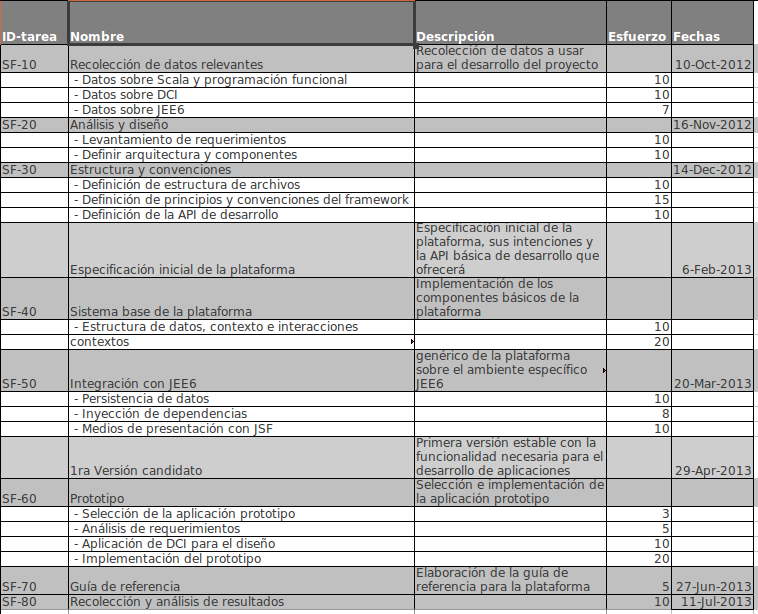
\includegraphics[width=16cm,height=13cm]{planning.png}}
	  \caption{Planificaci\'on temporal}
	\end{figure}
  \newpage


\section*{Novedad del trabajo}
\addcontentsline{toc}{section}{Novedad del trabajo}
  
  La visi\'on de una arquitectura de sistemas gen\'erica 
  puede ser aplicada a cualquier ambiente de desarrollo, 
  ya que las plataformas y herramientas usadas son detalles 
  del sistema y no definen lo que el sistema es ni lo que hace. 
  Tal arquitectura est\'a enfocada a dos aspectos importantes 
  en la industria de desarrollo, la correctitud de las aplicaciones 
  y la capacidad de las mismas de crecer y ser mantenibles. El 
  presente trabajo es un acercamiento a estos conceptos a trav\'es 
  de una herramienta de desarrollo concreta, con la cual es 
  posible elaborar sistemas cubriendo las falencias detalladas 
  en la situaci\'on problem\'atica.

\section*{Aporte del trabajo}
\addcontentsline{toc}{section}{Aporte del trabajo}
  
  El aporte del presente trabajo es tanto te\'orico como pr\'actico 
  ya que los temas en los que basa, \gls{DCI} y programaci\'on objeto-funcional, 
  son relevantes tanto para el \'area de ingenier\'ia 
  del software como para la industria de desarrollo, 
  y el artefacto resultante, una plataforma de desarrollo, 
  es una herramienta de prop\'osito
  general enfocada al desarrollo de aplicaciones reales en base 
  a las necesidades capturadas en una empresa activa en el medio. 


\chapter{Programaci\'on objeto-funcional}
  Los lenguajes de programaci\'on emergentes de momento son aquellos
  que mezclan los conceptos de dos paradigmas presentes en la
  industria del software desde los a\~nos setenta, la orientaci\'on a
  objetos y la programaci\'on funcional.
\\
\\
  Mientras que la programaci\'on orientada a objetos se basa en
  abstracciones encapsuladas (los objetos) como base de su paradigma,
  la programaci\'on funcional se centra en las funciones como
  ciudadanos de primer orden.

\section{Programaci\'on orientada a objetos}

  La programaci\'on orientada a objetos ha sido inmensamente exitosa. 
  Empezando desde Simula en los a\~nos 60 y Smalltalk en los 70, es ahora el
  paradigma de programaci\'on predominante. El principio y
  motivaci\'on b\'asica de la programaci\'on orientada a objetos es
  simple: \emph{todos los programas requieren alg\'un tipo de
    estructura}\citep{programmingScala}.
\\
\\
  La forma mas simple de ejemplificarlo es a colocar datos y
  operaciones en algun tipo de contenedor. El concepto base de la
  orientaci\'on a objetos es hacer que estos contenedores sean
  generales, de forma que puedan contener datos y operaciones, y
  \'estos a su vez puedan ser contenidos en otros contenedores
  similares o que sean usados como par\'ametros para operaciones.
\\
\\
  Estos contenedores son denominados \emph{objetos}. Allan Kay, el
  inventor de Smalltalk, remarc\'o que de esta forma el objeto m\'as
  simple tiene el mismo principio de construcci\'on que un ordenador:
  \emph{combina datos con operaciones bajo una interfaz uniforme y
    formalizada}.  A pesar de que los lenguajes orientados a objetos
  han sido el foco de atenci\'on por mucho tiempo, existen
  relativamente pocos lenguajes que siguieron este principio b\'asico
  de construcci\'on hasta su conclusi\'on l\'ogica. 
\\
\\
  Por ejemplo,
  muchos lenguajes admiten valores que no son objetos, como los tipos
  de datos primitivos en Java. O permiten campos y operaciones
  est\'aticas que no son miembros de ning\'un objeto. \'Estas
  desviaciones del concepto original han conllevado a agregar
  complejidad y limitar escalabilidad en los
  programas\citep{programmingScala}.

\section{Programaci\'on funcional}

  Las ideas de programaci\'on funcional son m\'as antiguas que los
  ordenadores electr\'onicos. Sus fundamentos se remontan al c\'alculo
  lambda de la iglesia de Alonzo de los a\~nos 30. El primer lenguaje
  funcional fu\'e Lisp, creado en los a\~nos 50. Otros lenguajes
  funcionales populares son Scheme, SML, Erlang, Haskell, OCaml y
  F\#. Durante d\'ecadas la programaci\'on funcional ha estado
  limitada a campos acad\'emicos, sin embargo, en a\~nos recientes la
  industria de desarrollo ha incrementado su intere\'es en estos
  lenguajes\citep{programmingScala}.
\\
\\
  La programaci\'on funcional se gu\'ia por dos ideas:

  \begin{enumerate}
   \item Las funciones son valores de primer nivel.  \\ En un lenguaje
     funcional una funci\'on es un valor con la misma importancia que
     una cadena o un entero. Se pueden usar funciones como argumentos
     para otras funciones, retornar funciones como resultados o
     relacionarlas a con variables. Tambi\'en es posible definir
     funciones dentro de funciones de forma nominal o an\'onima.

   \item Las operaciones de un programa deber\'ian mapear valores de
     entrada hacia valores de salida si modificar el estado de los
     datos.
  \end{enumerate}

\section{Scala}

  Scala es un lenguaje de programaci\'on compatible con Java que ha
  estado en desarrollo desde el a\~no 2001 en el laboratorio de
  m\'etodos de programaci\'on del EPFL\footnote{\'Ecole Polytechnique
    F\'ed\'erale de Lausanne} y p\'ublicamente liberado para la
  plataforma JVM\footnote{Java Virtual Machine} desde Enero del 2004,
  la actual versi\'on estable es la 2.8 y es considerada como estable
  para ambientes de producci\'on.
\\
\\
  Scala combina programaci\'on orientada a objetos y funcional en un
  lenguaje est\'aticamente tipado. Est\'a orientado a la
  construcci\'on de componentes y sistemas de componentes desde su
  concepci\'on a trav\'es de los siguientes
  postulados\citep{scalaIntro}:

  \begin{itemize}
   \item Los lenguajes de programaci\'on para componentes de software
     necesitan ser escalables en el sentido de que los mismos
     conceptos pueden describir tanto partes grandes como peque\~nas
     de un sistema. Por tanto se concentra en mecanismos de
     abstracci\'on, composici\'on y decomposici\'on en vez de
     elementos primitivos que a pesar de ser \'utiles en cierta escala
     de bajo nivel no lo son a nivel de componentes.

   \item El soporte escalable para componentes puede ser prove\'ido
     por un lenguaje de programaci\'on que unifica y generaliza la
     programaci\'on funcional y la orientada a objetos.

  \end{itemize}
\subsection{Caracter\'isticas}

  Este es un resumen de los principales aspectos de
  Scala\citep{scalaIntro}:
  
  \begin{itemize}
   \item Scala combina la programaci\'on funcional y la orientada a
     objetos en un lenguaje uniforme.

   \item Los programas en Scala son similares a los programas en Java
     ya que Scala puede interactuar indistintamente con cualquier
     c\'odigo escrito en Java.

   \item Scala tiene un modelo de objetos uniforme, en el sentido de
     que cada valor es un objeto y cada operaci\'on una llamada de
     m\'etodo.

   \item Scala es a su vez un lenguaje funcional en el sentido de que
     las funciones son valores de primera clase.

   \item Scala tiene conceptos uniformes y poderosos para tipos de
     datos y valores.

   \item Scala tiene un sistema de construcci\'on de objetos y traits
     modular basado en la composici\'on flexible de mixins.

   \item Scala permite la descomposici\'on de objetos en base a la
     identificaci\'on de patrones.

   \item Scala permite extensiones externas de componentes usando
     vistas.

   \item Scala es un lenguaje est\'aticamente tipado, esto significa
     que el sistema clasifica variables y expresiones de acuerdo a los
     valores que pueden alojar y/o computar.

   \item Scala es compilado, todo c\'odigo escrito en Scala es
     compilado como bytecode completamente compatible con la m\'aquina
     virtual de Java.

   \item Scala est\'a dise\~nado como lenguaje de alto nivel, eso
     quiere decir que se enfoca en resolver problemas de forma
     productiva, reduciendo la complejidad a trav\'es del uso de
     niveles uniformes de abstracci\'on.

  \end{itemize}

  \begin{figure}[!hbtp]
    \centerline{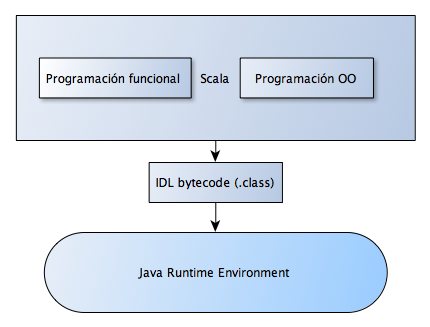
\includegraphics[height=7cm]{scala-overview.png}}
    \caption{Esquema general, Scala \citep{scalaIntro} }
  \end{figure}


%\subsection{Modelo de Objetos unificado}
%  TODO

\subsubsection{Clases y objetos}

  Las clases son notaciones est\'aticas que permiten definir elementos 
  con atributos, operaciones y estados. Los objetos son elementos 
  instanciados a partir de una clase, por ejemplo, el objeto Neo es 
  instancia de la clase Humano.
  
  Scala permite definir las clases de forma simplificada, una clase
  Java se definir\'ia as\'i:

  \begin{mylisting}
  \begin{verbatim}
  class MyClass {
      private int index;
      private String name;

      public MyClass(int index, String name) {
        this.index = index;
        this.name = name;
      }
    }
  \end{verbatim}
  \end{mylisting}

  y su equivalente en Scala es:

  \begin{mylisting}
  \begin{verbatim}
    class MyClass(index: Int, name: String)
  \end{verbatim}
  \end{mylisting}

  Y agrega un nuevo tipo de dato denominado \emph{objeto}, que es 
  un tipo de dato de instancia \'unica en el entorno de ejecuci\'on.

  \begin{mylisting}
  \begin{verbatim}
    object FindLongLines {
      def main(args: Array[String]) {
        val width = args(0).toInt
        for (arg <- args.drop(1))
          LongLines.processFile(arg, width)
        }
    }
  \end{verbatim}
  \end{mylisting}

\subsubsection{Funciones y m\'etodos}

  Las funciones son secuencias de \'ordenes ejecuci\'on 
  que tienen valores de entrada y salida, los m\'etodos son
  funciones que est\'an contenidas dentro de objetos. 

  Ya que la programaci\'on funcional define a las funciones 
  como elementos de primer orden, las funciones pueden ser parte 
  de otras funciones, ya sea de forma determin\'istica o an\'onima.

  \begin{mylisting}
  \begin{verbatim}
    def processFile(filename: String, width: Int) {
      def processLine(filename: String, width: Int, line: String) {
        if (line.length > width)
          println(filename +": "+ line)
      }
      val source = Source.fromFile(filename)
      for (line <- source.getLines()) {
        processLine(filename, width, line)
      }
    }
  \end{verbatim}
  \end{mylisting}
%\subsubsection{Variables y propiedades}
%  TODO
%\subsection{Operaciones}
%  TODO
%\subsubsection{M\'etodos y valores funcionales}
%  TODO
%\subsubsection{Funciones}
%  TODO
%\subsection{Abstracci\'on}
%  TODO
%\subsubsection{Abstracciones funcionales}
%  TODO
%\subsubsection{Miembros abstractos}
%  TODO
%\subsection{Composici\'on}
%  TODO

\chapter{Arquitectura DCI}

  La arquitectura de Datos, Contexto e Interacciones (DCI de sus siglas
  en ingl\'es, Data Context Interaction) es una arquitectura de
  sistemas ideada a lo largo de la carrera de Trygve Reenskaug, el
  creador del patr\'on de presentaci\'on
  Modelo-Vista-Controlador \footnote{MVC, Model View Controller}.

\begin{figure}[!hbtp]
  \centerline{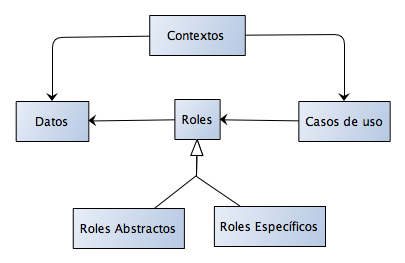
\includegraphics[height=6cm]{dci_overview.png}}
  \caption{Esquema DCI \citep{leanArchitecture} }
\end{figure}

  Ambos, DCI y MVC se orientan hacia la interacci\'on entre personas y
  m\'aquinas, mientras MVC \emph{separa las partes de un programa que
    son responsables de la representaci\'on de la informaci\'on en el
    sistema y las partes que son responsables de la interacci\'on con
    el usuario}, DCI \emph{minimiza cualquier brecha que pueda existir
    entre el modelo mental del programador de su programa y el
    programa que est\'a almacenado y siendo ejecutado en el
    ordenador. En particular, concreta el c\'omo el sistema realiza
    sus operations como una red de objetos en comunicaci\'on}
  \citep{leanArchitecture}.
\\
\\
  Simplificando el concepto de DCI, separa la arquitectura de un
  sistema en la parte de \emph{datos}( el dominio \'o lo que el
  sistema es) y en una \emph{interacci\'on} (lo que el sistema
  hace). La parte de datos se conecta con la parte de interacci\'on a
  trav\'es de una secuencia de eventos denominados el
  \emph{contexto}. La arquitectura puede ser vista como \emph{Datos} e
  \emph{Interacci\'on} din\'amicamente conectados a trav\'es de un
  \emph{Contexto} \citep{leanArchitecture}.

\section{DCI y MVC}
  El objetivo de DCI es separar el c\'odigo que representa el estado
  del sistema del c\'odigo que representa su comportamiento. Esta
  separaci\'on es similar pero diferente a la que realiza MVC.

\begin{figure}[!hbtp]
  \centerline{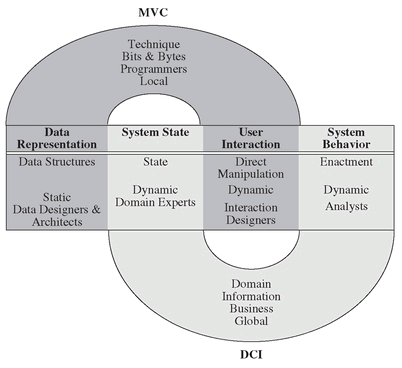
\includegraphics[width=9cm,height=9cm]{dci_arch2.png}}
  \caption{Relaci\'on entre DCI y MVC \citep{leanArchitecture}}
\end{figure}
 
  MVC y DCI est\'an dise\~nados para trabajar juntos como una forma
  de que los programadores razonen sobre el model mental del usuario y
  el c\'omo capturar esos modelos en el c\'odigo.

\section{Ejemplo pr\'actico}
  Tengamos el siguiente escenario en una entidad financiera:
  \begin{quote}

    \emph{Un banco en el cual se realizan los pagos al personal de
    diferentes niveles a trav\'es de la cuenta de su jefe de
    secci\'on, de manera manual a trav\'es de transferencias, requiere
    que este proceso que puede llegar a tomar 2 horas por secci\'on se
    automatice, de forma que el personal pueda enfocar su esfuerzo en
    tareas mas prioritarias.}
  \end{quote}

  En este escenario tenemos que el banco realiza transferencia entre
  cuentas, tales cuentas pueden ser de los gerentes de secci\'on como
  de los empleados, y la tarea a ejecutar es el pago de
  sueldos. Organizando todos estos elementos seg\'un la arquitectura
  DCI tenemos:

  \begin{itemize}
    \item \emph{Objetos del dominio}: Las cuentas bancarias, simples
      objetos con s\'olo los atributos y comportamientos b\'asicos de
      una cuenta.

    \item \emph{Roles}: Al ser las cuentas bancarias entidades
      b\'asicas de negocio, los roles definen el comportamiento de
      estos objetos para una o varias responsabilidades
      espec\'ificas. Para este caso, tenemos que las cuentas de
      empleados reciben el dinero, mientras que las cuentas de los
      gerentes transfieren dinero.

    \item \emph{Contexto}: El contexto viene a ser el evento en s\'i,
      el deposito de sueldos, lo que hace el contexto es crear cuentas
      y agregarles comportamiento de forma din\'amica, siendo los
      gerentes aquellos que depositan dinero a las cuentas
      empleado. No es posible que las cuentas empleados puedan
      realizar otras operaciones porque no tienen esas capacidades en
      este contexto, asimismo para las cuentas de gerentes, solamente
      tienen \emph{inyectado} el comportamiento necesario para
      realizar el dep\'osito de sueldos. De esta forma el dominio y la
      sem\'antica de la operaci\'on se reduce exactamente a lo que el
      usuario realmente quiere hacer.

  \end{itemize}

%glossary
\printglossary
%\addcontentsline{toc}{chapter}{Glosario de t\'erminos}
% bibliography
\bibliographystyle{plainnat}
\bibliography{biblio}
% annexes
\chapter*{Anexos}
\addcontentsline{toc}{chapter}{Anexos}

\section*{Anexo 1 - Curriculum Vitae}
\addcontentsline{toc}{section}{Anexo 1 - Curriculum Vitae}
\includepdf[pages={1,2}]{references/cv_timoteo_ponce.pdf}



\end{document}
